\documentclass[preview,border=4mm,convert={convertexe={magick},outext=.ps}]{standalone}
\usepackage[dvipdfm]{geometry}

%graphics
\usepackage{xcolor}
\usepackage{tikz}
\usepackage{pgfmath}
\usetikzlibrary{calc,arrows.meta}
\usepackage[caption=false,font=footnotesize]{subfig}

\begin{document}
\begin{figure}[!t]
\centering

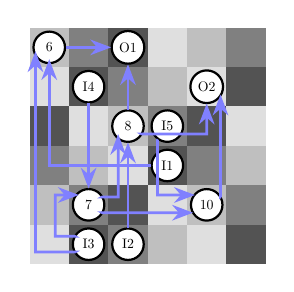
\begin{tikzpicture}[
scale=0.5,transform shape,
c1/.style={rectangle, fill, lightgray!50, minimum size=1cm},
c2/.style={rectangle, fill, lightgray, minimum size=1cm},
c3/.style={rectangle, fill, gray, minimum size=1cm},
c4/.style={rectangle, fill, darkgray!90, minimum size=1cm},
route/.style={->, >={Stealth[]},line width=1pt, blue!50},
v/.style={circle, draw, fill=white, line width = 0.8pt, minimum size=0.8cm},
]

%draw USE clock scheme
\def\sz{6}
\pgfmathparse{\sz-1}
\foreach \x in {0,1,...,\pgfmathresult}
  \foreach \y in {0,1,...,\pgfmathresult}
    \pgfmathparse{(mod(\y,2)!=0) ? ((mod(\y+1,4)!=0)?(1+mod(\x+1,4)):(1+mod(\x+3,4))):((mod(\y,4)==0)?(4-mod(\x+3,4)):(4-mod(\x+1,4)))}
    \pgfmathparse{int(\pgfmathresult)}
    \node[c\pgfmathresult]at(\x,\y){};
     
%draw area = 30;
\node(9)[v]  at (2,5){O1};
\node(6)[v]  at (0,5){6};
\node(11)[v] at (4,4){O2};
\node(8)[v]  at (2,3){8};
\node(10)[v] at (4,1){10};
\node(7)[v]  at (1,1){7};
\node(1)[v]  at (3,2){I1}; 
\node(2)[v]  at (2,0){I2};
\node(3)[v]  at (1,0){I3};
\node(4)[v]  at (1,4){I4};
\node(5)[v]  at (3,3){I5};

%如果结点设置为圆形
%左上45度 -- ++(-0.35,0.2)
%右上45度 -- ++(0.35,0.2)
%右下45度 -- ++(0.35,-0.2)
%左下45度 -- ++(-0.35,-0.2)
\draw[route] (3) -- ++ (-0.35,0.2)-- ++ (-0.5,0) -- ++(0,1.05) --++ (0.6,0);
\draw[route] (4) -- (7);
\draw[route] (5) -- ++ (-0.25,-0.35) -- ++ (0,-1.4) -- ++ (0.95,0);
\draw[route] (7) -- ++ (0.35,-0.2) -- ++ (2.3,0) ;
\draw[route] (2) -- (8) ;
\draw[route] (7) -- ++ (0.35,0.2) -- ++ (0.4,0) -- ++(0,1.6);
\draw[route] (8) -- ++ (0.35,-0.2) -- ++ (1.65,0) --(11) ;
\draw[route] (10) -- ++ (0.35,0.2) -- ++(0,2.6);
\draw[route] (1) -- ++ (-3,0) -- ++ (0,2.7) ;
\draw[route] (3) -- ++ (-0.35,-0.2) -- ++ (-1,0) -- ++ (0,5.1) ;
\draw[route] (6) -- (9) ;
\draw[route] (8) -- (9) ;

\end{tikzpicture}
\end{figure}
\end{document}
